%%%%%%%%%%%%%%%%%%%%%%%%%%%%%%%%%%%%%%%%%
% Thesis 
% LaTeX Template
% Version 1.3 (21/12/12)
%
% This template has been downloaded from:
% http://www.latextemplates.com
%
% Original authors:
% Steven Gunn 
% http://users.ecs.soton.ac.uk/srg/softwaretools/document/templates/
% and
% Sunil Patel
% http://www.sunilpatel.co.uk/thesis-template/
%
% License:
% CC BY-NC-SA 3.0 (http://creativecommons.org/licenses/by-nc-sa/3.0/)
%
% Note:
% Make sure to edit document variables in the Thesis.cls file
%
%%%%%%%%%%%%%%%%%%%%%%%%%%%%%%%%%%%%%%%%%

%----------------------------------------------------------------------------------------
%	PACKAGES AND OTHER DOCUMENT CONFIGURATIONS
%----------------------------------------------------------------------------------------

\documentclass[11pt, a4paper, oneside]{Thesis} % Paper size, default font size and one-sided paper

\graphicspath{{./Pictures/}} % Specifies the directory where pictures are stored

\usepackage[square, numbers, comma, sort&compress]{natbib} % Use the natbib reference package - read up on this to edit the reference style; if you want text (e.g. Smith et al., 2012) for the in-text references (instead of numbers), remove 'numbers' 
\hypersetup{urlcolor=blue, colorlinks=true} % Colors hyperlinks in blue - change to black if annoying
\title{\ttitle} % Defines the thesis title - don't touch this

\begin{document}

\frontmatter % Use roman page numbering style (i, ii, iii, iv...) for the pre-content pages

\setstretch{1.3} % Line spacing of 1.3

% Define the page headers using the FancyHdr package and set up for one-sided printing
\fancyhead{} % Clears all page headers and footers
\rhead{\thepage} % Sets the right side header to show the page number
\lhead{} % Clears the left side page header

\pagestyle{fancy} % Finally, use the "fancy" page style to implement the FancyHdr headers

\newcommand{\HRule}{\rule{\linewidth}{0.5mm}} % New command to make the lines in the title page

% PDF meta-data
\hypersetup{pdftitle={\ttitle}}
\hypersetup{pdfsubject=\subjectname}
\hypersetup{pdfauthor=\authornames}
\hypersetup{pdfkeywords=\keywordnames}

%----------------------------------------------------------------------------------------
%	TITLE PAGE
%----------------------------------------------------------------------------------------

\begin{titlepage}
\begin{center}

\textsc{\LARGE \univname}\\[1.5cm] % University name
\textsc{\Large Doctoral Thesis}\\[0.5cm] % Thesis type

\HRule \\[0.4cm] % Horizontal line
{\huge \bfseries \ttitle}\\[0.4cm] % Thesis title
\HRule \\[1.5cm] % Horizontal line
 
\begin{minipage}{0.4\textwidth}
\begin{flushleft} \large
\emph{Author:}\\
\href{http://www.johnsmith.com}{\authornames} % Author name - remove the \href bracket to remove the link
\end{flushleft}
\end{minipage}
\begin{minipage}{0.4\textwidth}
\begin{flushright} \large
\emph{Supervisor:} \\
\href{http://www.jamessmith.com}{\supname} % Supervisor name - remove the \href bracket to remove the link  
\end{flushright}
\end{minipage}\\[3cm]
 
\large \textit{A thesis submitted in fulfilment of the requirements\\ for the degree of \degreename}\\[0.3cm] % University requirement text
\textit{in the}\\[0.4cm]
\groupname\\\deptname\\[2cm] % Research group name and department name
 
{\large \today}\\[4cm] % Date
%
\includegraphics{Logo} % University/department logo - uncomment to place it
 
\vfill
\end{center}

\end{titlepage}

%----------------------------------------------------------------------------------------
%	DECLARATION PAGE
%	Your institution may give you a different text to place here
%----------------------------------------------------------------------------------------
% 
% \Declaration{
% 
% \addtocontents{toc}{\vspace{1em}} % Add a gap in the Contents, for aesthetics
% 
% I, \authornames, declare that this thesis titled, '\ttitle' and the work presented in it are my own. I confirm that:
% 
% \begin{itemize} 
% \item[\tiny{$\blacksquare$}] This work was done wholly or mainly while in candidature for a research degree at this University.
% \item[\tiny{$\blacksquare$}] Where any part of this thesis has previously been submitted for a degree or any other qualification at this University or any other institution, this has been clearly stated.
% \item[\tiny{$\blacksquare$}] Where I have consulted the published work of others, this is always clearly attributed.
% \item[\tiny{$\blacksquare$}] Where I have quoted from the work of others, the source is always given. With the exception of such quotations, this thesis is entirely my own work.
% \item[\tiny{$\blacksquare$}] I have acknowledged all main sources of help.
% \item[\tiny{$\blacksquare$}] Where the thesis is based on work done by myself jointly with others, I have made clear exactly what was done by others and what I have contributed myself.\\
% \end{itemize}
%  
% Signed:\\
% \rule[1em]{25em}{0.5pt} % This prints a line for the signature
%  
% Date:\\
% \rule[1em]{25em}{0.5pt} % This prints a line to write the date
% }
% 
% \clearpage % Start a new page

%----------------------------------------------------------------------------------------
%	QUOTATION PAGE
%----------------------------------------------------------------------------------------
% 
% \pagestyle{empty} % No headers or footers for the following pages
% 
% \null\vfill % Add some space to move the quote down the page a bit
% 
% \textit{``Thanks to my solid academic training, today I can write hundreds of words on virtually any topic without possessing a shred of information, which is how I got a good job in journalism."}
% 
% \begin{flushright}
% Dave Barry
% \end{flushright}
% 
% \vfill\vfill\vfill\vfill\vfill\vfill\null % Add some space at the bottom to position the quote just right
% 
% \clearpage % Start a new page

%----------------------------------------------------------------------------------------
%	ABSTRACT PAGE
%----------------------------------------------------------------------------------------

% \addtotoc{Abstract} % Add the "Abstract" page entry to the Contents
% 
% \abstract{\addtocontents{toc}{\vspace{1em}} % Add a gap in the Contents, for aesthetics
% 
% The Thesis Abstract is written here (and usually kept to just this page). The page is kept centered vertically so can expand into the blank space above the title too\ldots
% }
% 
% \clearpage % Start a new page

%----------------------------------------------------------------------------------------
%	ACKNOWLEDGEMENTS
%----------------------------------------------------------------------------------------
% 
% \setstretch{1.3} % Reset the line-spacing to 1.3 for body text (if it has changed)
% 
% \acknowledgements{\addtocontents{toc}{\vspace{1em}} % Add a gap in the Contents, for aesthetics
% 
% The acknowledgements and the people to thank go here, don't forget to include your project advisor\ldots
% }
% \clearpage % Start a new page

%----------------------------------------------------------------------------------------
%	LIST OF CONTENTS/FIGURES/TABLES PAGES
%----------------------------------------------------------------------------------------

\pagestyle{fancy} % The page style headers have been "empty" all this time, now use the "fancy" headers as defined before to bring them back

\lhead{\emph{Contents}} % Set the left side page header to "Contents"
\tableofcontents % Write out the Table of Contents
% 
% \lhead{\emph{List of Figures}} % Set the left side page header to "List of Figures"
% \listoffigures % Write out the List of Figures
% 
% \lhead{\emph{List of Tables}} % Set the left side page header to "List of Tables"
% \listoftables % Write out the List of Tables

%----------------------------------------------------------------------------------------
%	ABBREVIATIONS
%----------------------------------------------------------------------------------------

% \clearpage % Start a new page
% 
% \setstretch{1.5} % Set the line spacing to 1.5, this makes the following tables easier to read
% 
% \lhead{\emph{Abbreviations}} % Set the left side page header to "Abbreviations"
% \listofsymbols{ll} % Include a list of Abbreviations (a table of two columns)
% {
% \textbf{LAH} & \textbf{L}ist \textbf{A}bbreviations \textbf{H}ere \\
% %\textbf{Acronym} & \textbf{W}hat (it) \textbf{S}tands \textbf{F}or \\
% }

%----------------------------------------------------------------------------------------
%	PHYSICAL CONSTANTS/OTHER DEFINITIONS
%----------------------------------------------------------------------------------------

% \clearpage % Start a new page
% 
% \lhead{\emph{Physical Constants}} % Set the left side page header to "Physical Constants"
% 
% \listofconstants{lrcl} % Include a list of Physical Constants (a four column table)
% {
% Speed of Light & $c$ & $=$ & $2.997\ 924\ 58\times10^{8}\ \mbox{ms}^{-\mbox{s}}$ (exact)\\
% % Constant Name & Symbol & = & Constant Value (with units) \\
% }

%----------------------------------------------------------------------------------------
%	SYMBOLS
%----------------------------------------------------------------------------------------

% \clearpage % Start a new page
% 
% \lhead{\emph{Symbols}} % Set the left side page header to "Symbols"
% 
% \listofnomenclature{lll} % Include a list of Symbols (a three column table)
% {
% $a$ & distance & m \\
% $P$ & power & W (Js$^{-1}$) \\
% % Symbol & Name & Unit \\
% 
% & & \\ % Gap to separate the Roman symbols from the Greek
% 
% $\omega$ & angular frequency & rads$^{-1}$ \\
% % Symbol & Name & Unit \\
% }

%----------------------------------------------------------------------------------------
%	DEDICATION
%----------------------------------------------------------------------------------------

% \setstretch{1.3} % Return the line spacing back to 1.3
% 
% \pagestyle{empty} % Page style needs to be empty for this page
% 
% \dedicatory{For/Dedicated to/To my\ldots} % Dedication text
% 
% \addtocontents{toc}{\vspace{2em}} % Add a gap in the Contents, for aesthetics

%----------------------------------------------------------------------------------------
%	THESIS CONTENT - CHAPTERS
%----------------------------------------------------------------------------------------

\mainmatter % Begin numeric (1,2,3...) page numbering

\pagestyle{fancy} % Return the page headers back to the "fancy" style

% Include the chapters of the thesis as separate files from the Chapters folder
% Uncomment the lines as you write the chapters

\chapter{Introduction}
\label{chap:introduction} 
\lhead{Chapter \ref{chap:introduction}. \emph{Introduction}}

This chapter presents the general idea of this work. Section~\ref{intro:motivation} describes the motivation for optimization of resource allocation on the cloud. Section~\ref{intro:application} discusses the model of scientific applications. Section~\ref{intro:cloud} describes cloud business models and services that are used to deploy applications. Section~\ref{intro:statement} states the goals of the thesis. Section~\ref{intro:statement} enumerates challenges to be overcomed. 

\section{Motivation}
\label{intro:motivation}
\todo{Dodac jakies ladne zdanie na poczatek (``juz starozytni Rzymianie\ldots)}
This thesis illustrates typical problems when making decisions on deployment planning of scientific applications on IaaS clouds and how they can be addressed using optimization techniques. In contrast to already well established computing and storage resources (clusters, grids) for the research community, clouds in the form IaaS  platforms (pioneered by Amazon EC2) provide on-demand resource provisioning with a pay-per-use model. These capabilities together with the benefits introduced by virtualization, make clouds attractive to the scientific community~\cite{Deelman09}. As a result, multiple deployment scenarios differing in costs and performance, coupled together with new provisioning models offered by clouds make the problem of resource allocation and capacity planning for scientific applications a challenge.

\todo{dodac podsekcje Motivation gdzie beda challenges}


\section{Scientific applications}
\label{intro:application}

Nowadays, science requires processing of large amounts of data and use of hosted services for compute-intensive tasks\cite{Foster06052005}. Scientific computing covers a wide range of fields including biology, chemistry, economics, engineering, finance, geophysics, linguistics, mathematics, mechanics and physics. Applications used in this sciences are often distributed, so that application may run a numbers of magnitude faster than sequential one. This is very important in some fields such as weather forecasting or financial modelling to get results as fast as possible. 

Scientific applications often belong to one of the groups: 
\begin{itemize}
  \item workflow,
  \item bag of tasks,
  \item map\-reduce,  
  \item sequential batche,
  \item High Performance Computing application.
\end{itemize}

In this thesis we will focus on resource allocation for workflows and bag of tasks applications.

\subsection{Workflows}
\label{intro:workflow}

Scientific workflow is concerned with the automation of scientific processes in which tasks are structured based on their control and data dependencies\cite{Taylor:2006:WES:1196459}. Workflow application is composed by connecting multiple scientific tasks to their dependencies. Workflow structure indicates the temporal relationship between there tasks. In general, a workflow can be represented as a Directed Acyclic Graph (DAG) or a non-DAG. 

Workflow is built of four base control structures: \emph{sequence}, \emph{parallelism}, \emph{choice} and \emph{loop} (only for non-DAGs). Sequence represents an ordered series of task with one starting after the previous task has completed. Parallelism represents tasks that are performed concurrently, rather than serially. The choice structure allows to run selected portion of the workflow if certain conditions are met. The iteration structure lets certaint block of tasks to be repeated. Consecutive stages of workflow often represent work of scientist – data gathering, preprocessing, processing and results aggregation. 

In terms of scientific computing we will be rather interested in data flow in workflow. It is composed of the follwing structures (Figure~\ref{fig:intro:workflow:structures}): \emph{process}, \emph{pipeline}, \emph{data distribution}, \emph{data aggregation} and \emph{data redistribution}.

\begin{figure}[tb]
   \centering
   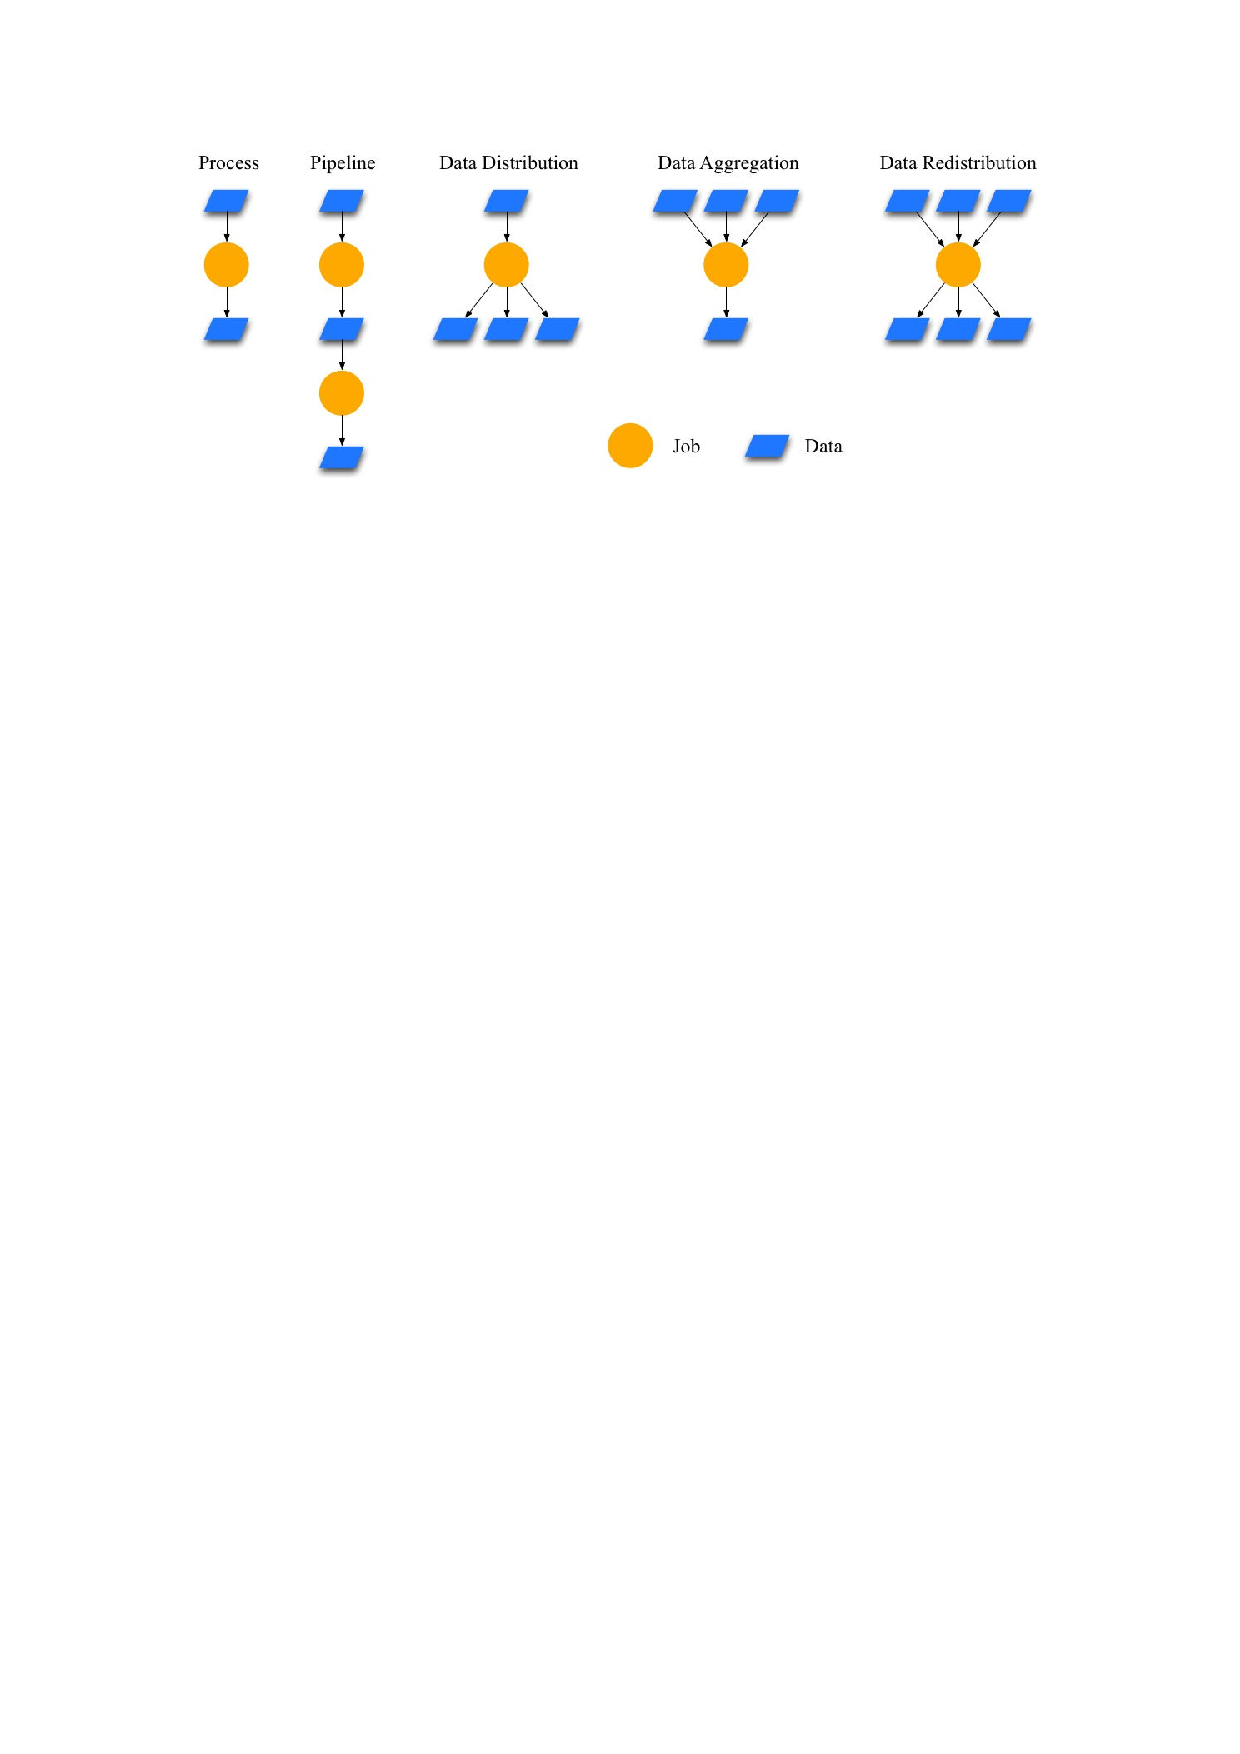
\includegraphics[width=\columnwidth]{WorkflowDataFlow}  
   \caption{Data flow structures in Workflows\cite{Bharathi08}}
   \label{fig:intro:workflow:structures}
\end{figure} 


\begin{figure}[tb]
   \centering
   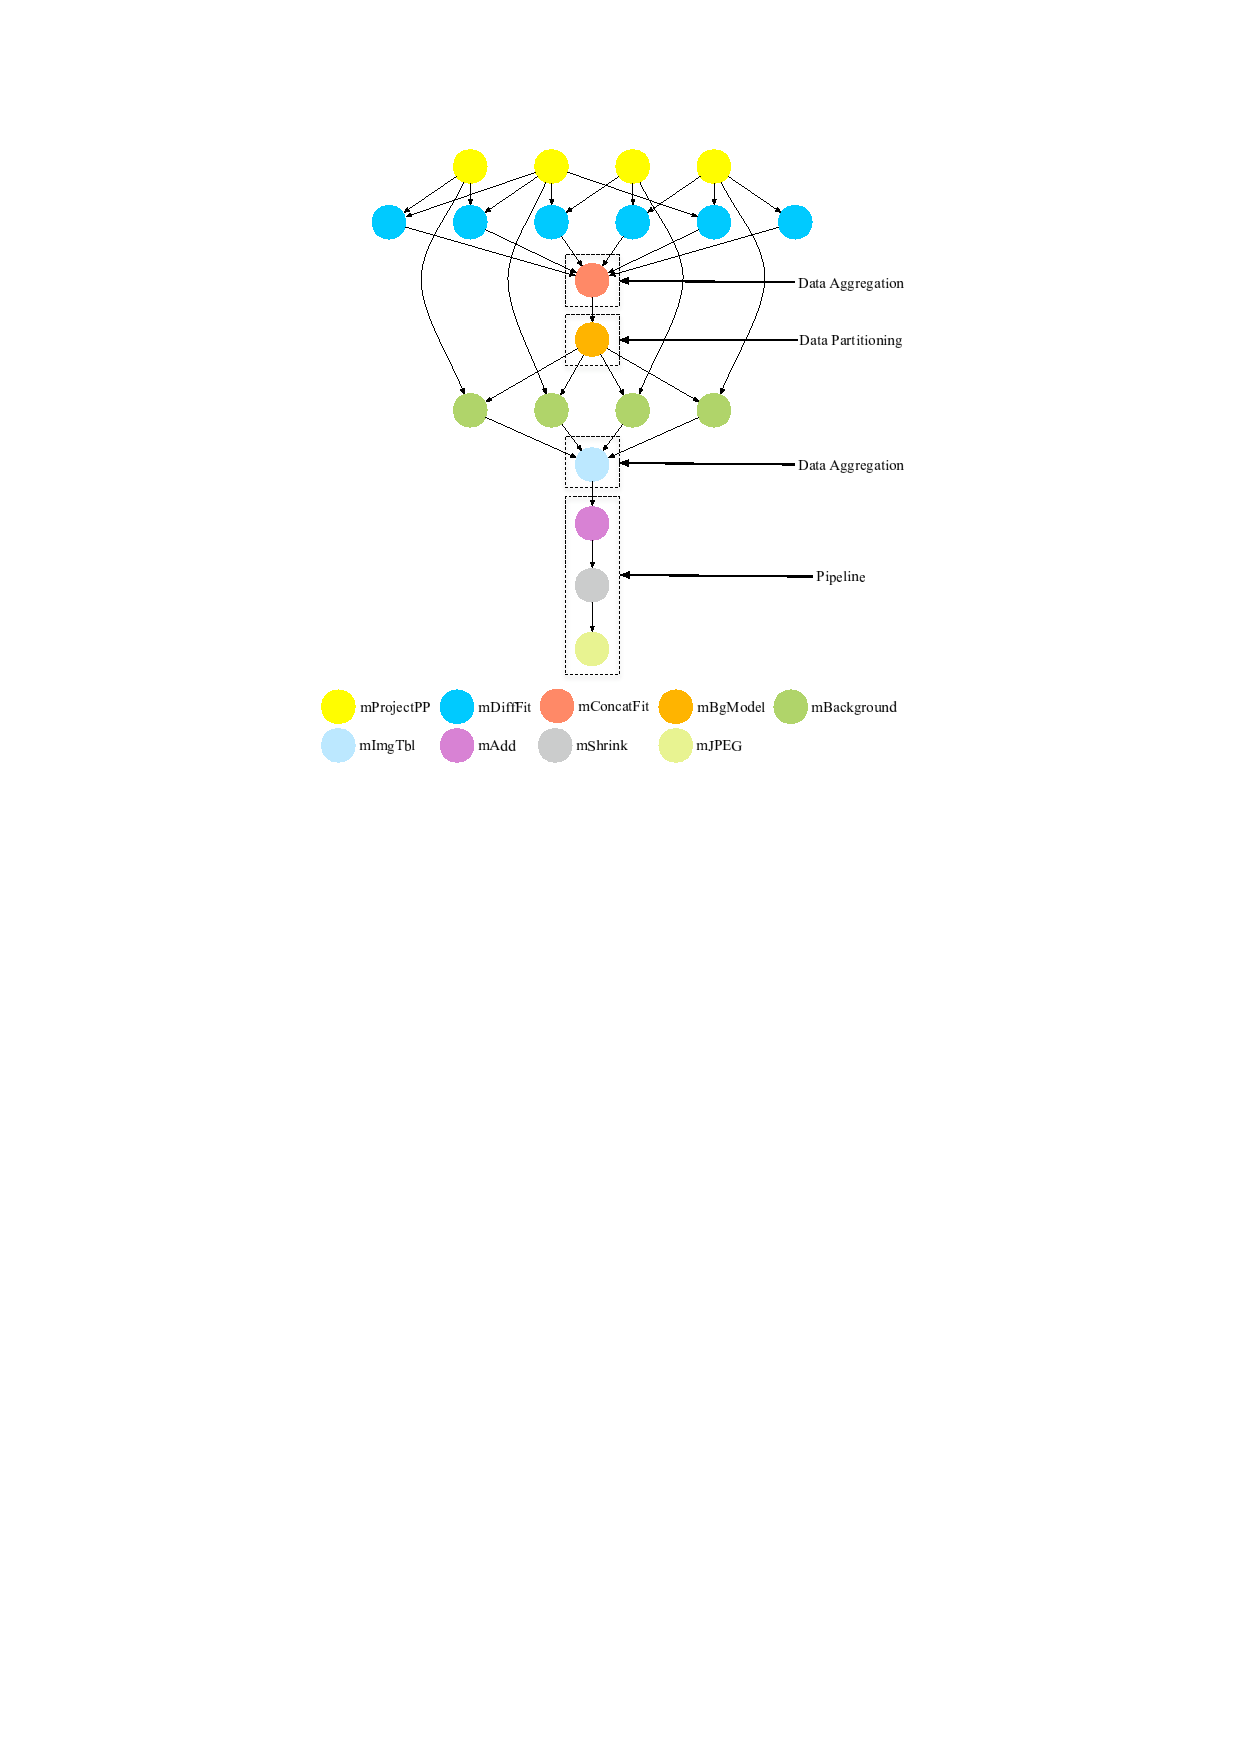
\includegraphics[width=0.7\columnwidth]{MontageWorkflow}  
   \caption{Montage – example workflow\cite{Bharathi08}}
   \label{fig:intro:workflow}\todo{Add reference to the figure in the text}
\end{figure} 

Scientific workflows are usually run on shared infrastructure as clusters, grids or clouds. It requires to carefully plan and schedule computation to efficiently use given infrastructure. As the workflows are getting bigger and more complex it is nearly impossible to do it manually. Specifically, scheduling workflow applications in a distributed system is an NP-complete problem\cite{Garey:1979:CIG:578533}. Numerous workflow algorithms to schedule workflows are presented in Chapter \ref{chap:state-of-art}.

There exist multiple workflow systems that assist scientists to create and deploy their workflow. Popular ones are Pegasus\cite{Pegasus} and Taverna\cite{Taverna}. They provide tools to model workflow either in code or via GUI application. Then one is able to generate workflow execution plan on certain (e.g. grid) architecture. Workflow systems differ in supported workflow types (DAG or non-DAG), workflow scheduling policies and algorithms, fault tolerance, and supported infrastructure. The good overview on workflow systems taxonomy is given in \cite{Yu:2005:TSW:1084805.1084814}.

\subsection{Bag of tasks}

Bag of tasks applications represent group of independent tasks that may be processed in parallel or sequentially. A large parameter sweep is good example of such problem. The \emph{map} stage of map-reduce\cite{Dean:2008:MapReduce} \todo{obrazek} application can be also considered as a bag of tasks. Additionally, many workflows include a stages of a high number parallel tasks. Such examples can be found e.g. in typical scientific workflows executed using Pegasus Workflow Management system, where e.g. CyberShake or LIGO workflows have a parallel stage of nearly homogeneous tasks~\cite{Bharathi08}. Other examples are Wien2K and ASTRO workflows that consist of iteratively executed parallel stages comprising homogeneous tasks\cite{Duan12}. Due to the high number of parallel branches, these stages accumulate the most significant computing time of the whole application, so optimization of the execution of this stage is crucial.


\section{Introduction to Cloud Computing}
\label{intro:cloud}

\todo{lepiej zaczac od tego, ze problem jest wazny i ciekawy.}Cloud computing is a jargon term without a commonly accepted non-ambiguous scientific or technical definition. The term is frequently used for marketing of hosted services or applications running in client-server model. As defined by US National Institute of Standards and Technology\cite{NISTCloudDef}, cloud computing is "a model for enabling ubiquitous, convenient, on-demand network access to a shared pool of configurable computing resources (e.g., networks, servers, storage, applications, and services) that can be rapidly provisioned and released with minimal management effort or service provider interaction".

\subsection{Service models}

We may categorize cloud services in terms of service model that give different level of control and responsibilities to user and service provider:

\begin{description}
  \item[Software as a Service (SaaS).] The capability provided to the user is to use applications deployed by provider running on a cloud infrastructure. The applications are usually available by web-browser based interface or program interface. The underlying cloud infrastructure including network, servers, operating system and application are managed by service provider. Popular SaaS applications include Gmail, Evernote and Salesforce CRM.
  \item[Platform as a Service (PaaS).] The capability provided to the user is to deploy his own appliactions created using programming languages, libraries, services and tools provied by the provider. The consumer does not manage underlying cloud infrastructure including network, servers, operating systems, runtime environment, but has control over the deployed application and configuration settings for cloud enviromnent. Example platforms include Heroku, Google App Engine and Nodejitsu.
  \item[Infrastructure as a Service (IaaS).] The capability provided to the user is to provision processing, storage, networks and other fundamental computing resources where the consumer is able to deploy and run arbitrary software. The consumer does not manage the underlying hardware infrastructure, but has control over operating system, storage, deployed appliations and has possibly limited control over networking (i.e. hosts firewall). Example platforms include Amazon EC2 and Rackspace.
\end{description}

\subsection{Deployment models}

Depending on who manages cloud infrastructure we may distinguish the following models:

\begin{description}
  \item[Private Cloud.] The cloud resources are provisioned for exclusive use by a single organization.
  \item[Community Cloud.] The cloud resources are provisioned for exclusive use by specific community of consumers from organization that have shared concerns. This is similar to scientific grid systems.
  \item[Public Cloud.] The cloud resources are provisioned for open use by the general public.
  \item[Hybrid Cloud.] The cloud infrastructure is composed of two or more distinct cloud providers that remain unique entities, but are bound together by technology that enables data and application portability. This technique is used for cloud bursting and offloading peak load to public cloud while using private resources when off-peak times.
\end{description}

\subsection{IaaS compute cloud}

Usually IaaS clouds provide three types of resources that are provisioned with a pay-per-use model: 
\begin{description}
  \item[Computing.] Provided as virtual machine (VM) instances. Multiple instance types are available that differ with CPU power, RAM memory and additional hardware (i.e. GPU units). VMs are usually billed for instance running time (wall clock time, not CPU time) usually rouned up to full hours.
  \item[Storage.] Provided as virtualized disk drives for virtual machines (i.e. Amazon's EBS) or as object store available as external service (i.e. Amazon's S3). User is usually biled for persisting data per GiB\footnote{Gibibyte $= 2^{30}$ bytes} per month. Additional charges may also apply (i.e. per IO transaction).
  \item[Networking.] Provides connectivity between VMs, storages and the Internet. User is billed for the data transfered of the cloud, while incoming data and transfer inside specific cloud usually remains free. Networking is provided in bundle with computing and storage, not as a separate service.
\end{description}

\section{Problem statement}
\label{intro:statement}

\todo{nalezy tu uzyc sformulowania 'resource allocation' zeby byc zgodnym z tytulem pracy} In this thesis we will focus on how planning and scheduling of bag of tasks and workflow applications. Planning scientific experiments requires optimization decisions that take into account both execution time and cost, as well as external constraints. Specifically, we will address the cost optimization problem of large-scale applications running on multiple heterogeneous clouds, using mathematical modeling with AMPL and mixed integer programming.

\section{Goals of the thesis}
\label{intro:goals}

The major goal of this thesis is the theoretical and practical investigation of optimization of resource allocation on the cloud by using integer linear programming tools and methods. In particular we are concerned with the following questions:

\begin{itemize}
  \item 
  \item Is it possible to perform such optimization by using AMPL?
  \item If so, is the optimization process fast enough and stable?
\end{itemize}

\todo{Dodac sekcje ``Goals of the thesis'' gdzie bedzie wypunktowana lista celow: analiza problemu, opracowania modelu, testy, itp. Pozniej w ostatnim rozdziale powinna byc ta sama lista i przy kazdym punkcie wyjasnione w jaki sposob cele zostaly zrealizowane.}

\chapter{State of the art review} \label{chap:state-of-art}  \lhead{Chapter 2. \emph{State of Art}}
 
Cloud computing is widely adopted standard for deploying web applications. Cloud users are charged on \emph{pay as you go} basis that enables for cost and service quality optimization by dynamic application scaling. Traditionally, in parallel and distributed systems like clusters and grids, workflow scheduling has been aimed to optimize the makespan or the time of completing all tasks~\cite{HEFT}. However, in context of cloud computing, the user needs to take care not only about makespan, but also about the financial cost of deploying application. Therefore, resource allocation on the cloud becomes a multi-objective optimization problem where no single optimal solution exists.

The problem of resource provisioning in IaaS clouds has been recently addressed in~\cite{Chen2011, Kim2011} and~\cite{SqueezingOut}. They typically consider unpredictable dynamic workloads and optimize the objectives such as cost, runtime or utility function by autoscaling the resource pool at runtime. In~\cite{Chen2011} they address semi-online resource provisioning for processing tasks with dynamic cloud pricing where users bid for the resources (e.g. Amazon EC2 Spot Instances).  On the other hand in~\cite{Kim2011} they consider workload offloading to the cloud from grid resources under deadline or budget constraint. In~\cite{SqueezingOut} they evaluate utility-based policy and reactive policies for dynamic resource provisioning. These approaches, however, do not address the problem of data transfer time and cost, which are an important factor when deploying scientific applications.

Automatic cloud scaling and provisioning is often delivered as a cloud service i.e. Amazon Auto Scaling\footnote{http://aws.amazon.com/autoscaling/}. Policy or rule based services are primarily designed to scale web applications~\cite{SqueezingOut} or bag of tasks applications (e.g.~\cite{ElasticSite, Kim2011}). They take input from monitoring systems and perform scaling-up or scaling-down depending on data from monitoring system. This approach is reasonable for applications with dynamic, unpredictable load as it allows to keep number of instances low, but high enough to provide certain service quality e.g. ensure acceptable request processing time.

The work presented in this thesis is related to heuristic algorithms for workflow scheduling on IaaS clouds, such as the ones described in~\cite{Abrishami2013158,Mao11,BarrionuevoFP12,BittencourtM11}. In~\cite{Abrishami2013158} the model assumes that infrastructure is provided by only one provider. In contrast, this work presents optimization on hybrid, multi-provider cloud. Infrastructure model considered differs in that we assume multiple heterogeneous clouds with object storage attached to them, instead of individual machines with peer-to-peer data transfers between them. Instead of scheduling each task individually, this approach proposes a global optimization of placement of workflow tasks and data.

Integer programming approach has been applied to the optimization of service selection for activities of QoS aware grid workflows~\cite{Brandic08}. On the other hand, in model presented in this thesis assumes the IaaS cloud infrastructure, while the objective function takes into account costs and delays of data transfers associated with the tasks.

The cost minimization problem on clouds addressed in~\cite{Pandey2010} uses a different model from ours. We impose a deadline constraint and assume that the number of instances available from providers may be limited. To satisfy these constraints, the planner has to choose resources from multiple providers. Our model also assumes that VM instances are billed per hour of usage.

The model presented in~\cite{Genez2012} also uses AMPL/CPLEX as solving platform and they define model for deadline-constrained workflow cost optimization. However, their approach does not address the problem of data transfer time and cost. Furthermore, they do not consider that number of instances on the cloud is usually limited. 

Pipelined workflows consisting of stages are addressed in~\cite{TolosanaCalasanz20121300}, where the processing model is a data flow and multiple instances of the same workflow are executed on the same set of cloud resources. The goal of this work is cost optimization instead of meeting the QoS constraints.

The deadline-constrained cost optimization of scientific workloads on heterogeneous IaaS described in~\cite{VandenBossche2013973} addresses multiple providers and data transfers between them, where the application is a bag of tasks.

\section{Summary}

None of the solutions presented in this chapter solves the problem we stated in Chapter~\ref{chap:introduction}. They solve other problems such as scheduling on only one cloud platform, or they are missing important parts of cost estimation (e.g. data transfer cost). So that, the problem of resource allocation on hybrid cloud platforms is still open. 
\chapter{Mathematical programming using AMPL}
\label{chap:ampl} 
\lhead{Chapter \ref{chap:ampl}. \emph{Mathematical programming using AMPL}}

Section \ref{sec:ampl:mathprog} presents overview on mathematical programming and problem classification (Section \ref{sec:ampl:classification}). In section \ref{sec:ampl:ampl} AMPL and other tools for mathematical programming are introduced. Then in Section \ref{sec:ampl:whiskas} we formulate example models: linear \emph{Whiskas Cat Food Problem} and integer \emph{shift work scheduling}.

\section{Mathematical Programming}
\label{sec:ampl:mathprog}

Nowdays, the term programming\cite{Programming} means writing software, but in 1940s this word was used to describe planning and scheduling activities. It appeared then that restrictions in the planning or scheduling problem may be represented mathematically using equalities and inequalities.  The solution satysfying all these constraints would be considered as acceptable plan or schedule.  Mathematical programming enables us to formally define optimization problem: it's varialbes, objective and constraints.

Defining the problem is not an easy task. If there are too few constraints, the space of possible solutions is too big. On the other hand, too many constraints can rule desirable solutions out. In the worst case there are no solutions at all. The success of programming relies on key insight into the optimized domain and modelling techniques to find a way round the possible difficulty. 

In addition to the constraints, one can define the objective --- function of the variables that makes it possible to compare solutions and select the best one. It doesn't matter how many solutions satisfy the constraints --- we are interested in the one that minimizes or maximizes the objective.

In development of optimization model it is very important to classify the problem, so we can select the most suitable way of solving it. If constraints and objectives are linear combinations of the variables then the model is called \emph{linear program} and the process of modelling and solving is called \emph{linear programming}. This class of optimization problems is particurarly important becasue a lot of real world optimization problems may be represented in such way. Additionally, there exists a lot of theory and algorithms to solve such problems in fast, deterministic way even if they have thousands of variables. The ideas of linear programming are also important for analyzing and solving problems that are non-linear.

All useful methods of mathematical programming involve using computers. The first computional method of solving optimization problems, the simplex algorithm, was introduced at that time and was subject to several improvements over the decades.

\section{Problem classification}
\label{sec:ampl:classification}

In spite of the broad applications of linear programming, the linearity assumption is too unrealistic to be applied to many of real problems. If instead smooth non-linear functions of the variables are used in constraints and objectives we call the program as \emph{non-linear program}. Solving such problems is much harder, but not impossible.

There is also another class of problems called \emph{integer programming} that assumes that variables are integer and in general it is much harder than previous. Fortuanetly, computational power of computers is still increasing and there are efficient algorithms to deal with them.

The optimization problems may be categorized in the following groups:
\begin{description}
  \item[Linear programming (LP)] Objective and constraints in this class are linear functions. Problems in this groups are usually solved by using \emph{simplex}, \emph{interior} or \emph{barrier} method.
  \item[Quadratic programming (QP)] Convex or concave objective and linear constraints. Solved by simplex-type or interior-type method.
  \item[Non-linear programming (NLP)] Continuous, but not all-linear objective and constraints. May be solved by several methods including gradient, quasi-newton, augmented lagrangian and interior-point. Unless special conditions are met, solution found is possibly optimal over only some local neighbourhood. If objective is convex (if minimized) or concave (if maximized) and constraints define a convex region it is guaranteed that optimum found is optimal over the entire feasible region.
  \item[Mixed-integer programming (MIP)] Linear objective and constraints, some or all of variables are integer-valued. Solved by branch-and-bound approach that uses a linear solver to solve subproblems.
  \item[Mixed-integer non-linear programming (MINLP)] Non-linear objective and constraints, some or all of variables are integer-valued. Solved by branch-and-bound approach that uses a non-linear solver to solve subproblems.
  \item[Constraint programming (CP)] \emph{TODO: pisac o tym w ogole?}\todo{tak :)}
\end{description}

\section{AMPL: A Mathematical Programming Language}
\label{sec:ampl:ampl}

To successfully solve optimization problem one needs to do a sequence of multiple tasks as follows:

\begin{enumerate}
  \item Formulate an abstract model: define variables, constraints and objective.
  \item Collect the data for a specific problem instance.
  \item Generate instance-specific variables, constraints and objective.
  \item Solve the problem by running a program called solver that implements algorithm that finds optimal solution.
  \item Analyze the results.
  \item Refine the model and the data as necessary, and repeat.
\end{enumerate}

Unfortuanetly, usually people use diffrent form of representing the data than algorithms do. This makes formulation and generation phases complex as modeller would like to express constraints in human-readable language e.g. mathematical notation, and solvers require to provide multiple matrices as input. We need to transform \emph{modeller's form} to \emph{algorithm's form}. Doing it manually is time consuming and erron-prone task.

To automate this task matrix generators were created for specific models. Altough they successfully automate matrix generation they are hard to code, debug and maintain. Modeller needs to be both mathematician and programmer. The other way to solve that problem is to use mathematical modelling language. Several languages\footnote{i.e. AMPL\cite{Fourer2002}, Gams\cite{Gams}, PuLP\cite{PuLP}, OscaR\cite{OscaR}} were created over the decades. 

By using modelling language, modeller may express in comfortable way also designed to serve as input for the computer. Then matrix generation may be fully automated without intermediate state of computer programming, thus mathematical programming becomes cheaper and more reliable. Benefits of formulating in modelling languages become particuraly advantageous for models being developed and subject to change.

AMPL is an algebraic mathematical modelling lanuage that resembles traditional mathematical notation to describe variables, objectives and constraints. Code in AMPL will be familiar for anybody that studied basic algebra or calculus, so that he or she doesn't need to be programmer (in present meaning). Algebraic modelling languages allow to express a wide range of optimization problems: linear, nonlinear and integer.

\subsection{Available solvers}

As soon as model is formulated and matrices generated, we may proceed with solving the specific instance of our problem. To do that we will need solver -- a program that implements one of solving algorithms. There is wide range of existing solvers available, both open-source (i.e. Cbc\cite{cbc-solver}) and commercial (i.e. CPLEX\cite{cplex}) ones that differ with the problem classes they target. Full list of available solvers is published at AMPL website\cite{AMPLSolvers}.

Usually solvers provide multiple options that let us tune them for the specific application. One may enable or disable certain features of the solver, i.e. for \emph{Bonmin}\cite{Bonmin} solver we may choose branching algorithm or configure it to use heuristics.

\section{Example -- Whiskas Cat Food Problem}
\label{sec:ampl:whiskas}
% zaczerpniete mocno z http://twiki.esc.auckland.ac.nz/twiki/bin/view/OpsRes/WhiskasCatFoodProblem

To get some practise with modelling, we will describe a typical linear programming problem on the example of Whiskas Cat Food problem. This is typical planning problem that may be found in many textbooks~\cite{dantzig}. \todo{Add non-breaking space (tilde) to all citations} The company producing the food wants to produce it as cheaply as possible while ensuring they meet the stated nutritional analysis requirements stated on the cans. 

Main ingredients of the cat food used are chicken, beef, mutton, rice wheat and gel. The prices for the ingredients are presented in Table \ref{ampl:whiskas:prices}, while ingredient contribution to the total weight of protein, fat, fibre and salt in the final product are give in Table \ref{ampl:whiskas:contribution} and nutritional requirements are presented in Table \ref{ampl:whiskas:analysis}. Given that data we may proceed with model formulation.

\begin{table}
  \centering
  \begin{tabular}{| l | r |}
    \hline
    \textbf{Ingredient} & \textbf{Price per gram} \\ \hline
    Chicken & \$ 0.013 \\ \hline
    Beef & \$ 0.008 \\ \hline
    Mutton & \$ 0.010 \\ \hline
    Rice & \$ 0.002 \\ \hline
    Wheat & \$ 0.005 \\ \hline
    Gel & \$ 0.001 \\ \hline
  \end{tabular}
  \caption{Cat food ingredient's pricing.}
  \label{ampl:whiskas:prices}  
\end{table}

\begin{table}
  \centering
  \begin{tabular}{| l | r | r | r | r |}
    \hline
    & \textbf{Protein} & \textbf{Fat} & \textbf{Fibre} & \textbf{Salt} \\ \hline
    \textbf{Chicken} & 0.100 & 0.080 & 0.001 & 0.002 \\ \hline
    \textbf{Beef} & 0.200 & 0.100 & 0.005 & 0.005 \\ \hline
    \textbf{Mutton} & 0.150 & 0.110 & 0.003 & 0.007 \\ \hline
    \textbf{Rice} & 0.000 & 0.010 & 0.100 & 0.002 \\ \hline
    \textbf{Wheat bran} & 0.040 & 0.010 & 0.150 & 0.008 \\ \hline
    \textbf{Gel} & -- & -- & -- & -- \\ \hline
  \end{tabular}
  \caption{Ingredient contribution to the final product in grams per gram of ingredient.}
  \label{ampl:whiskas:contribution}  
\end{table}

\begin{table}
  \centering
  \begin{tabular}{| l | r |}
    \hline
    Minimum \% Crude Protein & 8.0 \\ \hline
    Minimum \% Crude Fat & 6.0 \\ \hline
    Maximum \% Crude Fibre & 2.0 \\ \hline
    Maximum \% Salt & 0.4 \\ \hline
  \end{tabular}
  \caption{Cat food nutritional analysis.}
  \label{ampl:whiskas:analysis}  
\end{table}


  
\subsection{Problem formulation}

In this particular problem data defines the following data sets:

\begin{itemize}
  \item $I = \left\{\text{chicken}, \text{beef}, \text{mutton}, \text{rice}, \text{wheat}, \text{gel}\right\}$ -- defines possible ingredients,
  \item $C = \left\{\text{protein}, \text{fat}, \text{fibre}, \text{salt}\right\}$ -- defines components of nutrition.
\end{itemize}

We have also some numbers that describe members of sets;
\begin{itemize}
  \item $p_i$ -- price of given ingredient $i$ in \$ per gram
  \item $c_i,c$ -- contribution of ingredient $i$ to component of nutrition $c$ in grams per gram of ingredient.
\end{itemize}

\paragraph{Identify the decision variables}

First of all we need to identify decision variables. For the Whishas Cat Food Problem the descisions are the amounts of each ingredient we put in the can. Formally we could write this as:
\begin{align} 
  x_i &= \text{ amount (g) of ingredient $i$  in a can of cat food}
\end{align} 

\paragraph{Formulate the Objective Function}

The objective for this problem is to minimize the total cost of ingredients per fan of cat food. We know the cost per gram of each ingredient and the amount is to be found.

\begin{align}
   \min \mathop\sum\limits_{i \in I} p_i x_i
\end{align}

\paragraph{Formulate the constraints}

The constraints for the Whiskas Cat Food are:

\begin{enumerate}
  \item The sum of the amounts must make up the whole can (i.e. 100 g).
  \item The stated nutritional analysis requirements are met.
\end{enumerate}

First of the constraints can is: 

\begin{align}
   \mathop\sum\limits_{i \in I} x_i = 100
\end{align}

The latter can be written as follows

\begin{align}
   \mathop\sum\limits_{i \in I} c_{i,protein} x_i \geq 8.0 \\
   \mathop\sum\limits_{i \in I} c_{i,fat} x_i \geq 6.0 \\
   \mathop\sum\limits_{i \in I} c_{i,fibre} x_i \geq 2.0 \\ 
   \mathop\sum\limits_{i \in I} c_{i,salt} x_i \leq 0.4 \\
\end{align}

or in more general way, we may define lower and upper bounds for each component of nutrition as $L_c$ and $U_c$, the values are presented in Table \ref{ampl:whiskas:bounds}. Constraint will be written as

\begin{align}
   \mathop\forall\limits_{c \in C} L_c \leq \mathop\sum\limits_{i \in I} c_{i,c} x_i \leq U_c \\
\end{align}

\begin{table}
  \centering
  \begin{tabular}{| l | r | r |}
    \hline
    \textbf{Component of nutrition} & \textbf{Lower bound} & \textbf{Upper bound} \\ \hline
    Protein & 8.0 & -- \\ \hline
    Fat & 6.0 & -- \\ \hline
    Fibre & 2.0 & -- \\ \hline
    Salt & -- & 0.4 \\ \hline
  \end{tabular}
  \caption{Bounds for contribution of component of nutrition in percent.}
  \label{ampl:whiskas:bounds}  
\end{table}



We have formulated general problem using mathematical notation. Now we will proceed with model problem formulation using AMPL.

\subsection{Problem formulation using AMPL}

AMPL enables us to separate model definition and instance specific data. Usually we create three files: model, data and calling script. In the model file we define the data we need to have: sets and parameters, objective and constraints. Then in data file we populate the sets and parameters with the numbers for the particular instance of the problem. Both model and data files are loaded from calling script that may do some pre or post processing.

\paragraph{Model formulation}

First of all, we should define the sets for the ingredients and components of nutrition. We create file called \texttt{whiskas.mod} that will contain abstract model of optimization: sets, parameters, constraints and objective.

\begin{lstlisting}
set INGREDIENTS;
set COMPONENTS;
\end{lstlisting}

Using sets we can define the decision variables
\begin{lstlisting}
var Amount {INGREDIENTS} >= 0;
\end{lstlisting}

and parameters for the costs, components of nutrition contribution, restrictions and can size.

\begin{lstlisting}
param Cost {INGREDIENTS} >= 0;
param Contribution {INGREDIENTS, COMPONENTS} >= 0;

param Lower {COMPONENTS} default -Infinity;
param Upper {c in COMPONENTS} >= Lower[c], default Infinity;

param CanSize >= 0;

\end{lstlisting}

and the objective function

\begin{lstlisting}
minimize TotalCost : sum {i in INGREDIENTS} Cost[i] * Amount[i];
\end{lstlisting}

Note that, for the bounds that are not set, we assume \emph{±Infinity}. Additionally, we define that \emph{Cost} and \emph{Contribution} parameters should be non negative -- AMPL provides also verification of parameter data.


Finally, we may define constraints

\begin{lstlisting}
subject to MeetRequirements {c in COMPONENTS}:
  Lower[c] <= sum {i in INGREDIENTS} Contribution[i, c] * Amount[i] <= Upper[c];
  
subject to FullCan: 
  sum {i in INGREDIENTS} Amount[i] = CanSize;
\end{lstlisting}

\paragraph{Providing data}

Now we can provide the model with the data. To do this we create the file \texttt{whiskas.dat}.

First of all we need to provide sets we defined in previous paragraph.
\begin{lstlisting}
set INGREDIENTS := CHICKEN BEEF MUTTON RICE WHEAT GEL;
set COMPONENTS  := PROTEIN FAT FIBRE SALT;
\end{lstlisting}

Then we populate parameters with the data.
\begin{lstlisting}
param     Cost :=
  CHICKEN 0.013
  BEEF    0.008
  MUTTON  0.010
  RICE    0.002
  WHEAT   0.005
  GEL     0.001
;

param     Lower :=
  PROTEIN 8.0
  FAT     6.0
;

param     Upper :=
  FIBRE   2.0
  SALT    0.4
;

param CanSize := 100;

param Contribution :
          PROTEIN   FAT FIBRE  SALT :=
  CHICKEN   0.100 0.080 0.001 0.002 
  BEEF      0.200 0.100 0.005 0.005 
  MUTTON    0.150 0.110 0.003 0.007 
  RICE      0.000 0.010 0.100 0.002 
  WHEAT     0.040 0.010 0.150 0.008 
  GEL       0.0   0.0   0.0   0.0   
;
\end{lstlisting} 

\paragraph{Running AMPL}

Now we are ready to solve the model we formulated with AMPL. For that, let's create file called \texttt{whiskas.run}.

First of all we should reset AMPL environment in case that specific AMPL instance was solving other model before. We can do it with command \texttt{reset}. Then we load model using command \texttt{model} that takes model file name as an argument. Next, we load data file using command \texttt{data}. We also need to tell AMPL which solver we would like to be used. In our case we will use CPLEX (\texttt{option solver cplex}). Finally, we call solver and present results. The full file will look like as follows.

\begin{lstlisting}
reset;

model whiskas.mod;

data whiskas.dat;

option solver cplex;
solve;

display Amount;
\end{lstlisting}

Now we may run run AMPL and see if the model is working and if so, what is the optimal solution.

\begin{lstlisting}
% ampl whiskas.run
CPLEX 12.4.0.1: optimal solution; objective 0.52
2 dual simplex iterations (0 in phase I)
Amount [*] :=
   BEEF  60
CHICKEN   0
    GEL  40
 MUTTON   0
   RICE   0
  WHEAT   0
;
\end{lstlisting}

In that case, it appears that it is cheapest to use beef and fill the rest of the can with gel.

\section{Example -- Shift Scheduling}
\label{sec:ampl:sched}
\todo{say that it is an example of integer problem}
In this section, we will formulate AMPL model for shift scheduling problem\cite{Fourer2002}. The factory is working in three shift work schedule, operating six days a week from Monday to Saturday. On Saturday there's no third shift as it would overlap with Sunday. There's a certain number of workers required for each shift: more workers are required during first shift and less during the others. Due to work time regulations not all shift combinations of 5 day working week are possible. In the case described we already identified \todo{this was not described earlier} that there are 126 shift schedules possible. The crew wages depend on the choosen schedule. We also want to limit number of different schedules used, workers may work in teams during planned week. The problem is to minimize the cost of running factory while meeting all regulatory constraints.

\subsection{Problem formulation}

In this particular problem data defines the following data 

\begin{itemize}
  \item $S$ -- set of shifts,  
  \item $W$ -- set of acceptable schedules.
\end{itemize}

We have also some numbers that describe work planning;
\begin{itemize}
  \item $p_w$ -- pay rate at schedule $w$,
  \item $r_s$ -- number of staff required at shift $s$,
  \item $n_{min}$ -- minimal number of workers on any schedule.
\end{itemize}

\paragraph{Identify the decision variables}

We need to decide if given schedule will be used and if so, how many workers should follow it. Formally we could write this as:
\begin{align} 
  u_w &= \text{binary; schedule $w$ should be used iif 1} \\
  n_w &= \text{integer; how many workers should use schedule $w$}
\end{align} 

\paragraph{Formulate the Objective Function}

The objective for this problem is to minimize the total cost of running factory.

\begin{align}
   \min \mathop\sum\limits_{w \in W} p_w n_w
\end{align}

\paragraph{Formulate the constraints}

The constraints are:

\begin{enumerate}
  \item The stated minimal number of workers on each shift is met.
  \item Each schedule, if used at all, is used by minimal number of workers.
\end{enumerate}

First of the constraints is: 

\begin{align}
   \mathop\forall\limits_{s \in S}
     \mathop\sum\limits_{w \in W: s \in W_w} n_w \geq r_s
\end{align}

The second can be written as follows

\begin{align}
   \mathop\forall\limits_{w \in W}
     n_{min} u_w \leq n_w \\
   \mathop\forall\limits_{w \in W}
     n_w \leq \left(\max\limits_{s \in W_w} r_s\right) u_w 
\end{align}

We have formulated general problem using mathematical notation. Now we will proceed with model problem formulation using AMPL.

\subsection{Problem formulation using AMPL}

After we formulated the abstract model we implement it in AMPL by following the same procedure as in previous section. 

\paragraph{Model formulation}

First of all, we should define the sets and parameters in model file.

\begin{lstlisting}
set SHIFTS;
param Nsched;
set SCHEDS = 1..Nsched;
set SHIFT_LIST {SCHEDS} within SHIFTS;

param rate {SCHEDS} >= 0;
param required {SHIFTS} >= 0;
param least_assign >= 0;
\end{lstlisting}

Using sets we can define the decision variables
\begin{lstlisting}
var Work {SCHEDS} >= 0 integer; 
var Use {SCHEDS} >= 0 binary;
\end{lstlisting}

and the objective function

\begin{lstlisting}
minimize Total_Cost: sum {j in SCHEDS} rate[j] * Work[j];
\end{lstlisting}

Finally, we may define constraints

\begin{lstlisting}
subject to Shift_Needs {i in SHIFTS}:
  sum {j in SCHEDS: i in SHIFT_LIST[j]} Work[j] >= required[i];
subject to Least_Use1 {j in SCHEDS}: 
  least_assign * Use[j] <= Work[j];
subject to Least_Use2 {j in SCHEDS}:
  Work[j] <= (max {i in SHIFT_LIST[j]} required[i]) * Use[j];
\end{lstlisting}

\paragraph{Providing data}

Now we can provide the model with the data. We provide the data we defined in previous paragraph.

\begin{lstlisting}
set SHIFTS := Mon1 Tue1 Wed1 Thu1 Fri1 Sat1
              Mon2 Tue2 Wed2 Thu2 Fri2 Sat2
              Mon3 Tue3 Wed3 Thu3 Fri3 ;

param rate  default 1 ;

param required :=  Mon1 100  Mon2 78  Mon3 52 
                   Tue1 100  Tue2 78  Tue3 52
                   Wed1 100  Wed2 78  Wed3 52
                   Thu1 100  Thu2 78  Thu3 52
                   Fri1 100  Fri2 78  Fri3 52
                   Sat1 100  Sat2 78 ;
                   
param least_assign  := 5;
param Nsched        := 126 ;

set SHIFT_LIST[  1] := Mon1 Tue1 Wed1 Thu1 Fri1 ;
set SHIFT_LIST[  2] := Mon1 Tue1 Wed1 Thu1 Fri2 ;
........
set SHIFT_LIST[126] := Tue2 Wed2 Thu2 Fri2 Sat2 ;
\end{lstlisting} 

\paragraph{Running AMPL}

\begin{lstlisting}
reset;
option omit_zero_rows 1;
model whiskas.mod;

data whiskas.dat;

option solver cplex;
solve;

display Work;
display Total_Cost;
\end{lstlisting}

Now we are ready to run the model and get the results.

\begin{lstlisting}
% ampl sched.run
CPLEX 12.4.0.1: optimal integer solution; objective 266
136 MIP simplex iterations
23 branch-and-bound nodes
Work [*] :=
  3   7
  6  28
 16   8
 18   8
 20  12
 29   7
 37  21
 61   5
 66   5
 78  24
 82  28
 91  12
100   8
102   6
112  28
118  24
122  30
126   5
;

Total_Cost = 266
\end{lstlisting}

Given that data we may assign schedules to the specific workers.

\section{Conclusions}

This chapter presented basics of mathematical optimization. We discussed briefly history of optimiation, classification of optimization problems and introduced tools for mathematical optimization using computers. We also shown the example problems and corresponding models that may be solved using AMPL.
 
\chapter{Problem formulation}
\label{chap:formulation} 
\lhead{Chapter 4. \emph{Problem formulation}}


\section{Model for bag of tasks}

\subsection{Input parameters}

\subsection{Auxliary parameters}

\subsection{Decision variables}

\subsection{Constraints}

\subsection{Search space size complexity - ????}

\emph{TODO: Tu bym napisał od czego zależy rozmiar uniwersum rozwiązań}

\emph{TODO: Trzeba napisać dlaczego zostało to zamodelowane tak, a nie inaczej i jakie triki zostały zrobione}

\section{Model for workflows}

\emph{Tutaj podobnie jak wyzej}
% \input{./Chapters/Chapter4} 
% \input{./Chapters/Chapter5} 
% \input{./Chapters/Chapter6} 
% \input{./Chapters/Chapter7} 

%----------------------------------------------------------------------------------------
%	THESIS CONTENT - APPENDICES
%----------------------------------------------------------------------------------------

\addtocontents{toc}{\vspace{2em}} % Add a gap in the Contents, for aesthetics

\appendix % Cue to tell LaTeX that the following 'chapters' are Appendices

% Include the appendices of the thesis as separate files from the Appendices folder
% Uncomment the lines as you write the Appendices

% % Appendix A

\chapter{Appendix Title Here} % Main appendix title

\label{AppendixA} % For referencing this appendix elsewhere, use \ref{AppendixA}

\lhead{Appendix A. \emph{Appendix Title Here}} % This is for the header on each page - perhaps a shortened title

Write your Appendix content here.
%\input{./Appendices/AppendixB}
%\input{./Appendices/AppendixC}

\addtocontents{toc}{\vspace{2em}} % Add a gap in the Contents, for aesthetics

\backmatter

%----------------------------------------------------------------------------------------
%	BIBLIOGRAPHY
%----------------------------------------------------------------------------------------

\label{Bibliography}

\lhead{\emph{Bibliography}} % Change the page header to say "Bibliography"

\bibliographystyle{unsrtnat} % Use the "unsrtnat" BibTeX style for formatting the Bibliography

\bibliography{Bibliography} % The references (bibliography) information are stored in the file named "Bibliography.bib"

\end{document}  